\documentclass{article}
\usepackage[a4paper, margin=0.75in]{geometry}
\usepackage{graphicx}
\usepackage{titlesec}
\usepackage{amsmath}
\usepackage{graphicx}
\usepackage{float}
\usepackage{booktabs}
\usepackage{array}  
\usepackage{rotating}
\usepackage{pifont} 
\usepackage{subcaption}
\usepackage{setspace}
\usepackage{hyperref}
\usepackage{natbib}  % 引用 BibTeX 需要 natbib 包
\usepackage{multirow} 
\usepackage{titlesec}
\usepackage{array} % 控制列宽
\usepackage{adjustbox} 
\usepackage{ragged2e} % 支持两端对齐
\bibliographystyle{chicago}  % 使用 Chicago (Author-Date) 引用格式

\begin{document}

\begin{titlepage}
    \centering
    \vspace*{2cm}
    {\Huge \textbf{Proposal of ChatGIS: GIS-Powered Natural Language Query System}} \\
    \vspace{1.5cm}
    \textbf{Group Name:} ChatDB 70 \\
    \textbf{Course:} DSCI 551 - Foundations of Data Science \\
    \textbf{Instructor:} Dr. Wensheng Wu \\
    \textbf{Institution:} Viterbi School of Engineering, University of Southern California \\
    \textbf{Date:} \today \\
    \vfill
    \textbf{Team Members:} \\
    - [Yucheng Liu] - [Project Designing, Data Collection, Document Writing] \\
    

    \vfill
    \textbf{Team Members Background:} \\
    \begin{justify}

        \textbf{Yucheng Liu} is a Master’s student in Spatial Data Science at USC with a strong background in computer science, geospatial data science, and deep learning. He specializes in knowledge distillation, cloud-based application development, and geospatial analytics. Proficient in Python, SQL, NoSQL, and GIS, he has experience with AWS, TensorFlow,  and ArcGIS Pro. His research focuses on knowledge distillation and multimodal learning in the physiological signals, with publications in ACM MM and IJCAI.
        
    \end{justify}

    \vfill
    \begin{justify}
        \textbf{Project Abstract} - This proposal presents a \textbf{GIS-powered natural language query system} called ChatGIS that integrates \textbf{PostGIS} and \textbf{LLMs} to allow users to retrieve geospatial data using natural language queries. The system translates user queries into \textbf{optimized SQL statements} that efficiently interact with a GIS database, enabling users to ask spatial questions such as \textit{``Where are the nearest electric vehicle charging stations?''} or \textit{``Find all Chinese restaurants within 5 km of my location.''}. ChatGIS levels up the accessibility and usability of geospatial data by leveraging \textbf{LLM-based query processing, spatial indexing, and GIS visualization tools}.
        \vfill
        \textbf{Keywords:} GIS, LLM, PostGIS, Natural Language Queries, Spatial Database, Geospatial Search, Route Optimization, OpenStreetMap, API Development, Spatial Indexing, Machine Learning, Location-Based Services
    \end{justify}

\end{titlepage}

\section{Introduction}

Geospatial databases provide powerful spatial analysis capabilities but often require SQL expertise to query effectively. This make the GIS system hard to use for the non-technical user. To address this issue, we propose ChatGIS, a \textbf{GIS-powered natural language query system} that integrates \textbf{PostGIS} and \textbf{LLMs} to allow users to retrieve geospatial data using natural language queries. The system translates user queries into \textbf{optimized SQL statements} that efficiently interact with a GIS database, enabling users to ask spatial questions such as \textit{``Where are the nearest electric vehicle charging stations?''} or \textit{``Find all Chinese restaurants within 5 km of my location.''}. ChatGIS levels up the accessibility and usability of geospatial data by leveraging \textbf{LLM-based query processing, spatial indexing, and GIS visualization tools}.

This project aims to integrate \textbf{Large Language Models (LLMs)} with \textbf{PostGIS}, enabling users to perform spatial queries in California using natural language. By translating user queries into SQL, the system facilitates intuitive geospatial searches and, if time permits, visualizes the results on the web. Additionally, we provide a \textbf{Flask API} to support seamless integration into third-party applications. Furthermore, we plan to explore cloud deployment to offer \textbf{Location-Based Services} to users, contingent on available time.

\section{Data Source}

In this project, we will use the \textbf{\href{https://www.openstreetmap.org}{OpenStreetMap (OSM)}} dataset as the primary data source. OSM is a collaborative project that collects and distributes geospatial data, and it is a popular choice for geospatial research and applications. OSM provides a rich set of features, including points of interest, roads, buildings, and natural features. OSM data is available in a variety of formats, including XML, PBF, and SHP. In this project, we will download the dataset in the California to build the GIS database.

\section{Implementation}
\subsection{System Overview}
% 总体架构,描述 LLM + GIS 的流程

The overview of the system is shown in Figure \ref{fig:system_overview}. The system consists of three main components: \textbf{Front-end} and \textbf{Back-end (including GIS database, LLM model, and server API)}. The front-end is responsible for user input, query processing, and visualization. The LLM model is responsible for translating the input into SQL statements, optimizing the queries, and feedbacking the results. The GIS database is responsible for storing and managing the geospatial data as well as the spatial analysis. The server API is responsible for providing a RESTful interface for the front-end and third-party applications to interact with the system.

\begin{figure}[H]
    \centering
    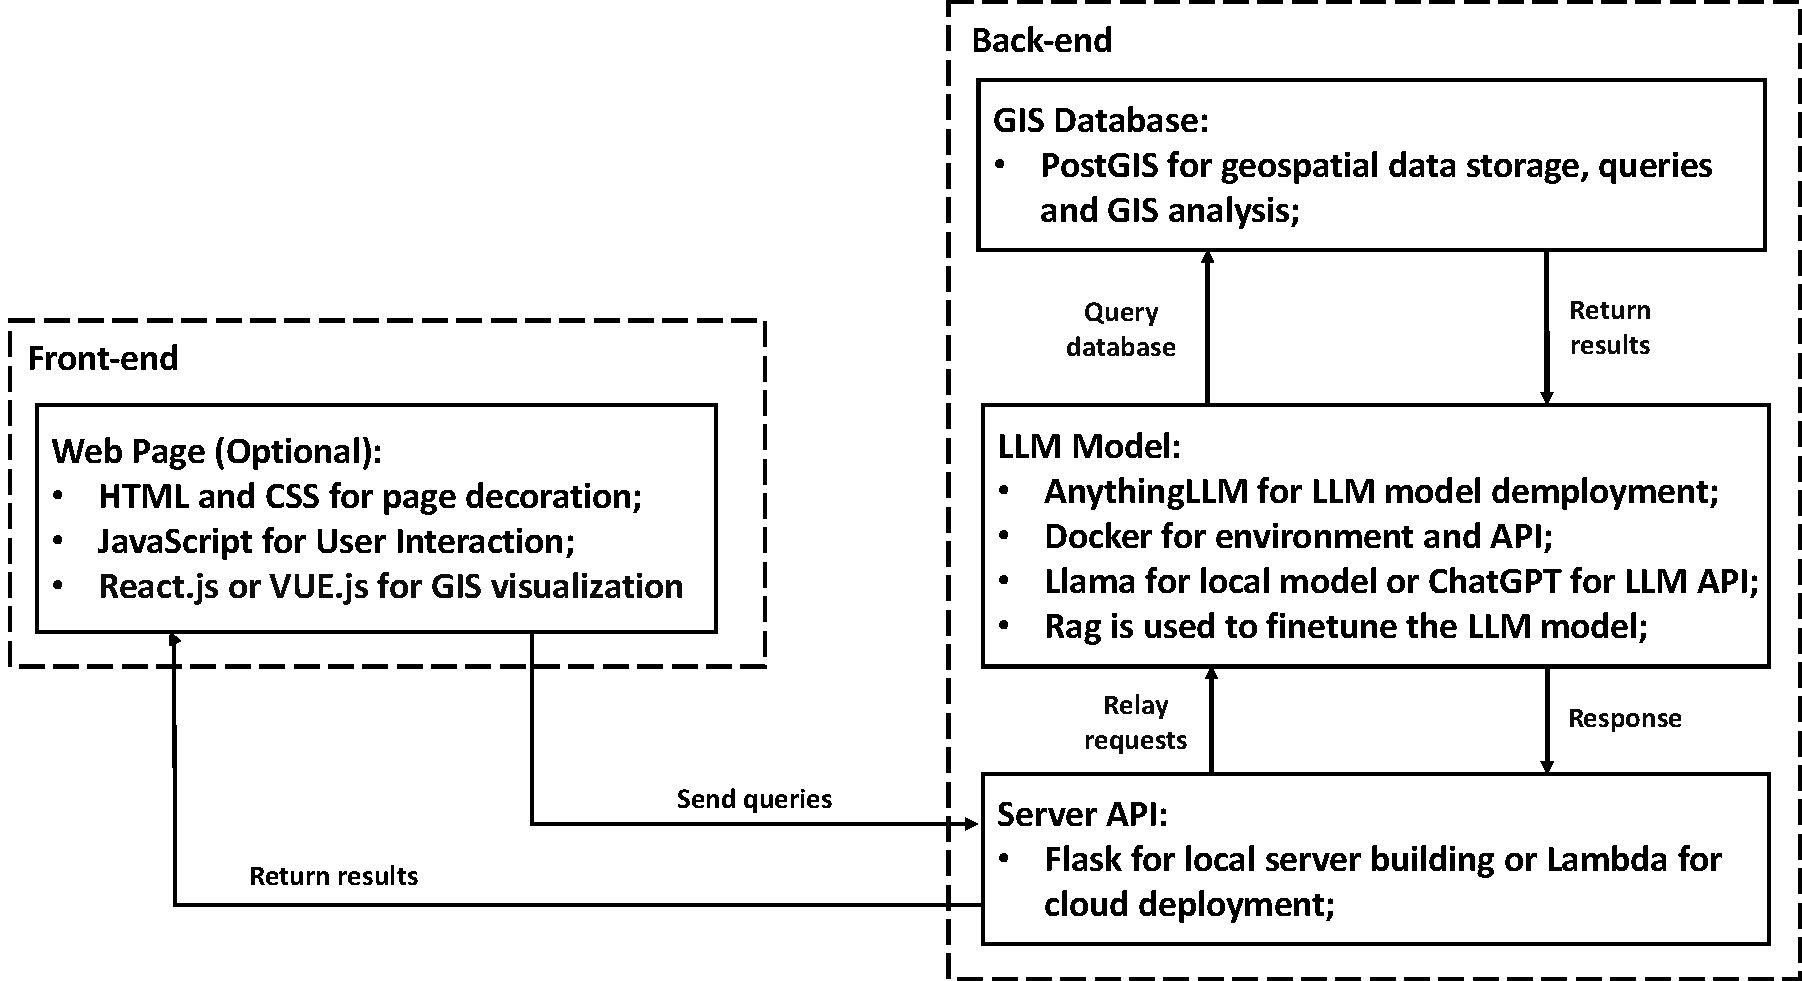
\includegraphics[width=0.8\textwidth]{figs/Overview.pdf}
    \caption{System Overview}
    \label{fig:system_overview}
\end{figure}

In this project, we will try to implement the local LLM model first and the LLM API (ChatGPT) second. Since this is the project for the single person, the front-end is the optional choice.  The GIS database will be built using the OSM dataset in California. The server API will be built using Flask and deployed locally if time permits, we may try to deploy the whole system to the cloud using AWS or Google Cloud Platform.

\subsection{LLM for Query Processing}
% LLM 如何解析用户查询并转换 SQL
In this project we will use the Llama model \cite{touvron2023llama} as the LLM locally. Llama is a natural language processing model developed by the Stanford NLP group. Llama is a pre-trained transformer-based language model that can generate SQL queries. We will use the Llama model to parse the user queries and convert them into SQL statements. The schema of the GIS database will be used in the Rag to help optimize the SQL queries.

ChatGPT \cite{achiam2023gpt} is a pre-trained transformer-based language model that can generate natural language responses. We will use the ChatGPT API as the Back up plan to generate responses to the user queries.

\subsection{Database \& Storage}
% PostGIS 数据结构、GIS 查询优化
In this project, we will use the PostGIS database \cite{obe2021postgis} to store and manage the geospatial data. PostGIS is a spatial database extender for PostgreSQL that adds support for geographic objects. The PostGIS database will be used to store and manage the geospatial data. The schema of the database will be designed based on the OSM dataset.

\subsection{API \& Integration}
% Flask API 如何提供服务

In this project, we will use Flask as the server API framework. Flask is a micro web framework written in Python. We will use Flask to provide a RESTful interface for the front-end and third-party applications to interact with the system. We will also provide a simple API endpoint to allow users to upload their own geospatial data to the system.

\subsection{Deployment Plan}
% 本地测试 vs. AWS 运行方式

In this project, we will deploy the system locally for testing first. We will use Docker to containerize the system and the database and provide a simple deployment script to allow users to quickly start the system. If time permits, we can deploy the whole system to the cloud using AWS or Google Cloud Platform.

\subsection{Visualization (Optional)}
% 基于 Web GIS 的可视化工具
In this project, we will use the ArcGIS Pro software as the visualization tool to check the results of the spatial queries and the layers downloaded from the OSM dataset. ArcGIS Pro is a geospatial software application that provides a wide range of GIS tools and visualization techniques. We will use the ArcGIS Pro to visualize the results of the spatial queries. Besides, we will also provide a simple visualization tool to allow users to visualize their own geospatial data. We will use the VUE.js to create a simple map visualization tool.


\section{Team Members \& Roles}

This is a single-person project. I will be responsible for the project design, data collection, document writing, project management, and the presentation of the project. I will also be responsible for the implementation of the system components and the integration of the components.

\section{Timeline}

Before the midterm submission, I plan to complete the following tasks:

\begin{enumerate}
    \item Design the project proposal and write the project report.
    \item Collect and clean the OSM dataset in California.
    \item Build the GIS database using the OSM dataset.
    \item Implement the local LLM model or the LLM API (ChatGPT).
\end{enumerate}
After the midterm and before the final submission, I plan to complete the following tasks:

\begin{enumerate}
    \item Implement the Flask API and integrate it with the front-end.
    \item Test the system locally and provide a simple deployment script.
    \item Write the final report and the presentation.
    \item Deploy the system to the cloud if time permits.
\end{enumerate}

% 参考文献部分
\bibliography{references}  % 引用 BibTeX 文件 "references.bib"

\end{document}